\documentclass{article}

\usepackage{tikz}

\author{Yeoun Chan Kim \and John Strauser \and Xuanang Wang}

\title{CS440 Report}

\begin{document}

\maketitle

\section*{Part 1}

\begingroup
\centering

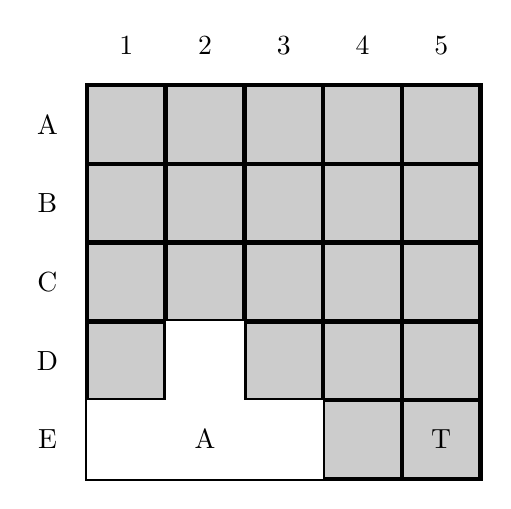
\begin{tikzpicture}
\draw [ultra thick, draw=black, fill=black!20!white] (0,0) grid  (5,5) rectangle (0,0);
\fill[white] (0,0) rectangle(1, 1);
\fill[white] (1,0) rectangle(2, 1); 
\fill[white] (2,0) rectangle(3, 1); 
\fill[white] (1,1) rectangle(2, 2); 
\node at (+1.5,+0.5) {A};
\node at (+4.5,+0.5) {T};
\node at (-0.5,+0.5) {E};
\node at (-0.5,+1.5) {D};
\node at (-0.5,+2.5) {C};
\node at (-0.5,+3.5) {B};
\node at (-0.5,+4.5) {A};
\node at (+0.5,+5.5) {1};
\node at (+1.5,+5.5) {2};
\node at (+2.5,+5.5) {3};
\node at (+3.5,+5.5) {4};
\node at (+4.5,+5.5) {5};
\end{tikzpicture}

\endgroup

\vspace{5mm} %5mm vertical space

a)Given the illustration above, Let (a, b) represent a unique state where a $\in$ \{ 1-5 \} and b $\in$ \{ A-E \}. We want to explain why the first move of the agent A in state (2, E) is to the east (3, E) rather than the north (2, D). Grey represents what agent cannot see and the white represents what agent can. According to the question, T in state (5, E) is the goal state. We calculate the Manhattan distance from A to T, which is 3 in the current situation: h(2, E) = 3. Let g(a, b)(c, d) represents the total distance cost from state (a, b) to state (c, d) in the A* searching path. Then in state (2, E), g(2, E)(2, E) = 0. Therefore, f(2, E) = 0 + 3 = 3. For all the state adjacent to (2, E) which are (1, E), (2, D), (3, E); the f value of each is (1, E): 4 + 1 = 5, (2, D): 4 + 1 = 5, (3, E): 2 + 1 = 3. According to the A* algorithm, we move the agent A to the position where the smallest f value holds. Therefore, the agent would move to the east (3, E) rather than the north(2, D) or (1, E).
\hspace{5mm}

b)Let S be the state in the finite gridworld, S{\small (s)} denotes the starting state, S{\small (c)} denotes the current state and S{\small (g)} denotes the goal state. For any S{\small (c)}, let h(S{\small (c)}) be the Manhattan distance from S{\small (c)} to S{\small (g)}, let g(S{\small (c)}) be the distance traveled from S{\small (s)} to S{\small (c)}, let S{\small (c')} be any adjacent state of S{\small (c)} and h(S{\small (c')}) g(S{\small (c')}) be the corresponding h and g value. According to the A* algorithm, for any state S{\small (c)}, as long as it's adjacent is not blocked which given value infinity, we calculate the f value using the formula f{\small (c')} = h(S{\small (c')}) + g(S{\small (c')}) and choose the one with the smallest f value. Because of the fact that for each iteration we always choose the {\tiny (min)}f{\small (c')} to be the next step for the path, as long as one of the possible path from S{\small (s)} to S{\small (g)} is not blocked, we would guarantee to reach the target. To make the explanation more clear, we consider the illustration below where black cells represent blocked.

\vspace{5mm} %5mm vertical space

\begingroup
\centering

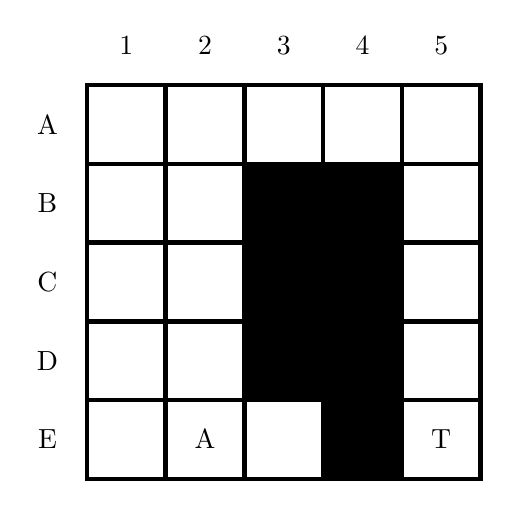
\begin{tikzpicture}
\draw [ultra thick, draw=black, fill=white] (0,0) grid  (5,5) rectangle (0,0);
\fill[black] (3,0) rectangle(4, 1);
\fill[black] (3,1) rectangle(4, 2); 
\fill[black] (3,2) rectangle(4, 3); 
\fill[black] (3,3) rectangle(4, 4); 
\fill[black] (2,1) rectangle(3, 2); 
\fill[black] (2,2) rectangle(3, 3); 
\fill[black] (2,3) rectangle(3, 4); 
\node at (+1.5,+0.5) {A};
\node at (+4.5,+0.5) {T};
\node at (-0.5,+0.5) {E};
\node at (-0.5,+1.5) {D};
\node at (-0.5,+2.5) {C};
\node at (-0.5,+3.5) {B};
\node at (-0.5,+4.5) {A};
\node at (+0.5,+5.5) {1};
\node at (+1.5,+5.5) {2};
\node at (+2.5,+5.5) {3};
\node at (+3.5,+5.5) {4};
\node at (+4.5,+5.5) {5};
\end{tikzpicture}

\endgroup

\vspace{5mm} %5mm vertical space

Because we are using the greedy approach, the next move of agent A at state (2, E) would be (3, E) (explained in part 1a)). However, when the state moves to (3, E), the dead-end situation occurred. Whenever we meet the situation like this, we would trace back to the parent cell of the dead ended cell, which is (2, E). After this, we would put (3, E) to closed list therefore the agent A would not able to go the (3, E) again even if f(3, E) is the smallest giving the situation the current state is (2, E).
\hspace{5mm}

However, if we put another block on (4, A), the agent would traverse from (2, E) vertically to (2, A); then go to (3, A) and backtrace to (2, A) because of the dead end.After that, the agent would go to (1, A) and vertically travel down to (1, E). In this situation, the open list is empty therefore the program returns false.

\end{document}